\documentclass{subfiles}

\begin{document}
	\section{Introduction}
	\par This section is a case study containing field work from a {\color{blue} non-forester perspective} to better understand the challenges of working remotely with forests. Remotely sensed data contain a great amount of information but in order to build a good system for identifying trees and materials, an in depth knowledge of them is required \cite{Smith2012}. For that reason, this case study was created; information about the New Forest, which is a forest in the south of United Kingdom, were collected and a small validation dataset was created. The dataset created includes the tree species and approximate heights of the trees in two areas of interest. 
	

	\par Before travelling to the New Forest, two areas of interest were selected. These areas were selected according to the following criteria:
	\begin{itemize}
		\item There were LiDAR data of the selected area to be able to compare what we can see on the ground with the scanned data
		\item Areas that had a variation of tree species were selected. This was done according to the (non-validated) results of a thesis of Bournemouth University that classified the tree species of the New Forest \cite{Sumnall2013}. This helped get a broader range of tree species. 
	\end{itemize}
	
	\par The following sections give a detailed description of the information gathered during the trip. This includes the species and height maps generated, the different types of landscapes found and the challenges faced. 
		
	
	   \section{Validation Data Collected}
	   \par The tree classes were initially defined by the provided Bournemouth thesis \cite{Sumnall2013}. A colour was chosen for each tree class and, while being in the New Forest, the aim was to mark each tree on the paper map with the corresponding colour. Using QGIS (Quantum Geographic Information System) the classification results of the forest assessment, undertaken by Sumnall in 2013 \cite{Sumnall2013}, were coloured with the same colours to ease comparison.
	   
	   \par At the aforementioned forest assessment, there were 26 classes from 14 different species; the remaining 12 classes were young versions of the 14 species. Here the classes are reduced to 14 by merging all the young trees into the tree species classes (in the 4 years gap between the 2010 assessment and and the visit to new Forest in 2014, the young trees would have aged).  See table \ref{tab:TBL_InitialColours} for the initial 14 classes. Nevertheless, more tree species existed in the areas of interest in New Forest than those 14 classes. The colours and symbols of the extra tree classes are shown on table \ref{tab:TBL_AddedColours}. 
	   
	   \begin{table}[!h]
	   	\centering
	   	\begin{tabular}{c}
	   		\raisebox{-\totalheight}{\adjincludegraphics[width=\linewidth]{img/NewForest/TBLInitialColours}}
	   	\end{tabular}
	   	\caption{Colours of the initial 14 classes}
	   	\label{tab:TBL_InitialColours}
	   \end{table}
	   
	   \begin{table}[!h]
	   	\centering
	   	\begin{tabular}{c}
	   		\raisebox{-\totalheight}{\adjincludegraphics[width=\linewidth]{img/NewForest/TBLAddedColours}}
	   	\end{tabular}
	   	\caption{Classes that were added during the trip}
	   	\label{tab:TBL_AddedColours}
	   \end{table}
	   
	   \par During the visit, tree species maps were generated for a few square meters. The position of the trees were found relative to easily-spotted refereence points (e.g. road crossing) that were marked in advanced. That was done because, according to Dr. Ross Hill, no GPS can be accurate enough when trees are around since the satellite signal bounces off the leaves and reduces the positioning accuracy. In professional fieldwork, a total station is used but, for the purposes of this visit, it was not considered necessary. By the end of the case study, ground maps were coloured according to the tree species identified and estimates of the approximate heights of the trees were also noted down. 
	   
	   \par The following four maps were created for each selected area. The first two maps were created before the trip during preparation, while the last two contain the information collected during the field work.
	   \begin{itemize}
	   	\item a screen shot of the area from Google map, 
	   	\item the classification results from the forest assessment \cite{Sumnall2013}, 
	   	\item the coloured tree species map and 
	   	\item the approximated height map.
	   \end{itemize}
	   
	   
	   \par Comparing the validation dataset created with the classifications done at Bournemouth University (which were not validated), it is clear there are misclassifications. This is shown in Figures \ref{fig:NF_Area1} and \ref{fig:NF_Area2} and it is likely that is occurs due to the over-segmentation of trees. Those wrong classifications justify that validation and field work data are essential for building a good classifier. 
	   
	   \newpage
	   \par The first area is included in the LAS file named LDR-FW-FW10\_01-201018715.LAS and it lies inside the limits:  X = (433453 - 433761), Y = (102193 - 102405) [British National Grid coordinates]. The four maps that relate to these areas are shown in Figure \ref{fig:NF_Area1}.
	   
	   \begin{figure} [h!]
	   	\begin{subfigure}[t]{.5\textwidth}
	   		\centering
	   		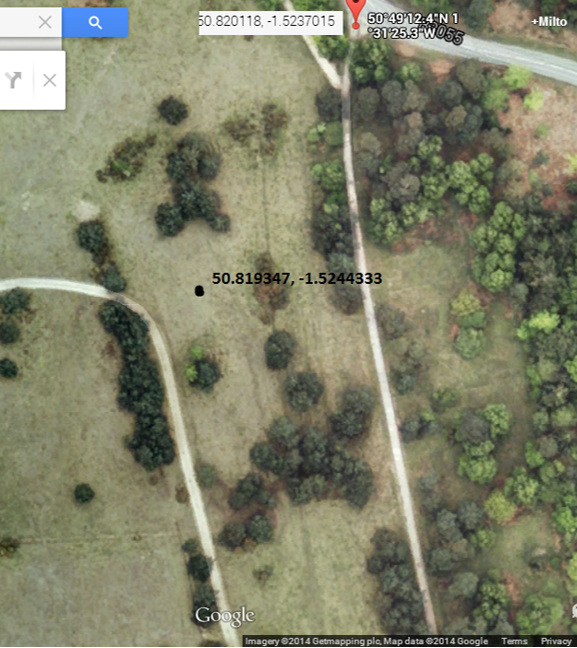
\includegraphics[width=.9\textwidth]{img/NewForest/Area1GoogleMap}
	   		\caption{Google map screenshot}
	   		\label{fig:Area1GoogleMap}
	   	\end{subfigure} \hfill
	   	\begin{subfigure}[t]{.5\textwidth}
	   		\centering
	   		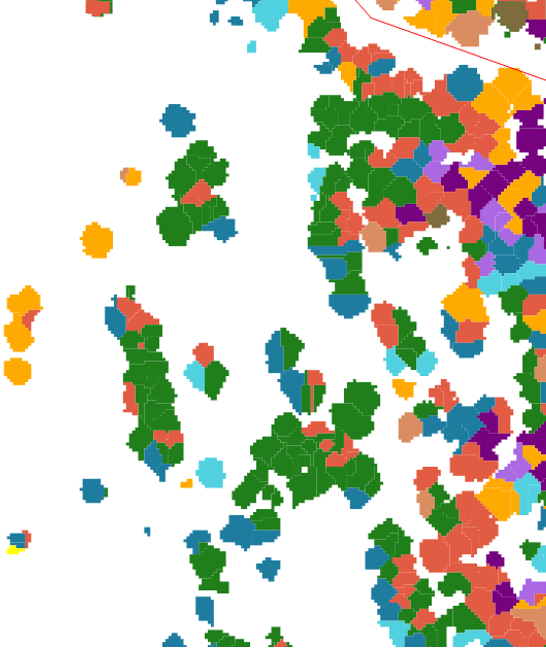
\includegraphics[width=.9\textwidth]{img/NewForest/Area1Classifications}
	   		\caption{Forest assessment classifications} 
	   		\label{fig:Area1Classifications}
	   	\end{subfigure}
	   	\begin{subfigure}[t]{.5\textwidth}
	   		
	   		\centering
	   		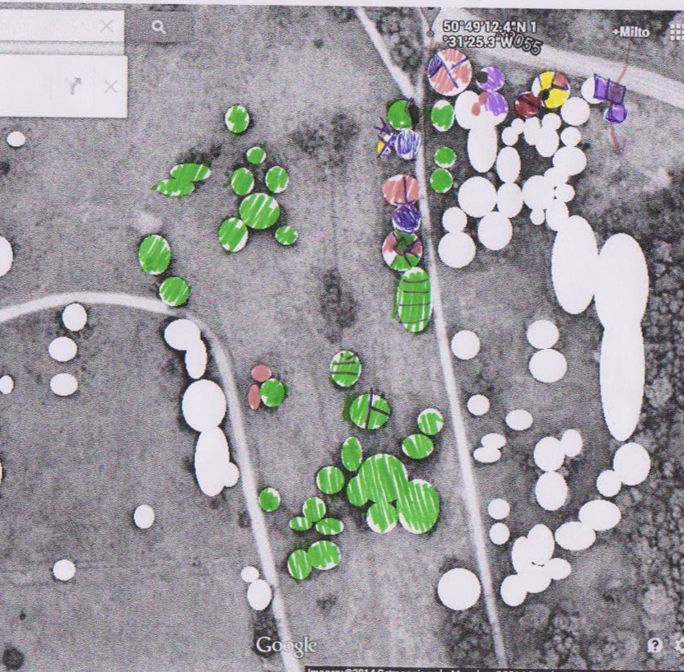
\includegraphics[width=.9\textwidth]{img/NewForest/Area1Fieldwork_Species}
	   		\caption{Tree species map, from field work}
	   		\label{fig:Area1Fieldwork_Species}
	   	\end{subfigure} \hfill
	   	\begin{subfigure}[t]{.5\textwidth}
	   		\centering
	   		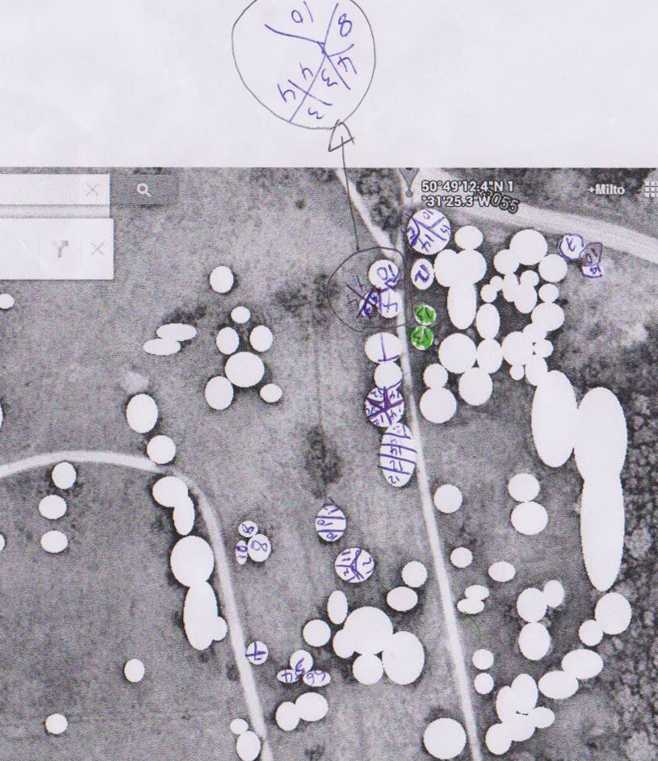
\includegraphics[width=.9\textwidth]{img/NewForest/Area1Fieldwork_Heights}
	   		\caption{Approximate heights of the trees, from field work} 
	   		\label{fig:Area1Fieldwork_Heights}
	   	\end{subfigure}
	   	\caption{The first area of interest and the related maps.} %\footnotemark[1].} 
	   	\label{fig:NF_Area1} 
	   \end{figure}
	   
	   
	   
	   \newpage
	   \par The second area is included in the LAS files named LDR-FW-FW10\_01-201018719.LAS and LDR-FW-FW10\_01-201018718.LAS and it lies inside the limits:  X = (436442 - 436835), Y = (102334 - 102585) [British National Grid coordinates]. The four maps created for these areas are shown in Figure \ref{fig:NF_Area2}.
	   
	   \begin{figure} [h!]
	   	\begin{subfigure}[t]{.5\textwidth}
	   		\centering
	   		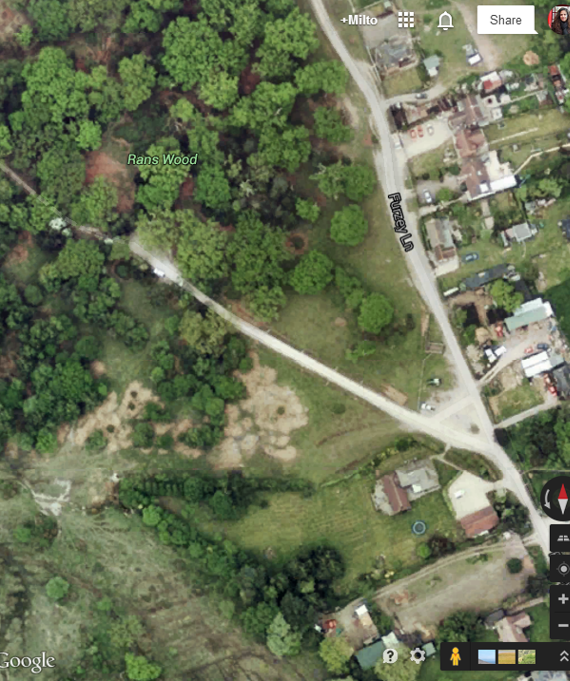
\includegraphics[width=.9\textwidth]{img/NewForest/Area2GoogleMap}
	   		\caption{Google map screenshot}
	   		\label{fig:Area2GoogleMap}
	   	\end{subfigure} \hfill
	   	\begin{subfigure}[t]{.5\textwidth}
	   		\centering
	   		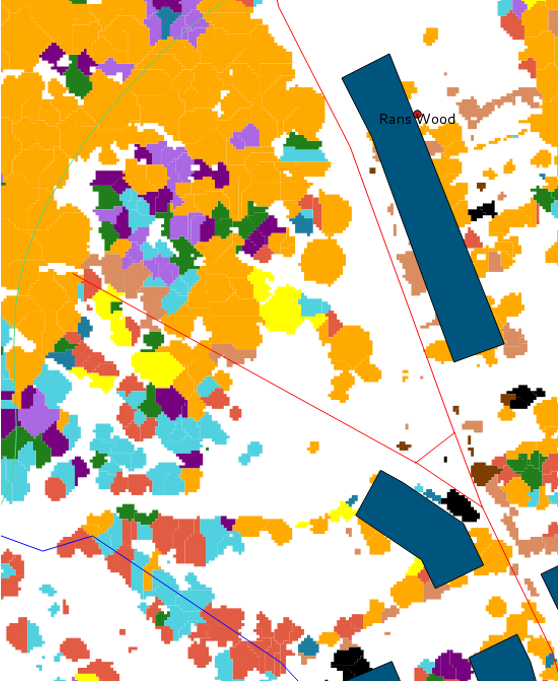
\includegraphics[width=.9\textwidth]{img/NewForest/Area2Classifications}
	   		\caption{Forest assessment classifications} 
	   		\label{fig:Area2Classifications}
	   	\end{subfigure}
	   	\begin{subfigure}[t]{.5\textwidth}
	   		
	   		\centering
	   		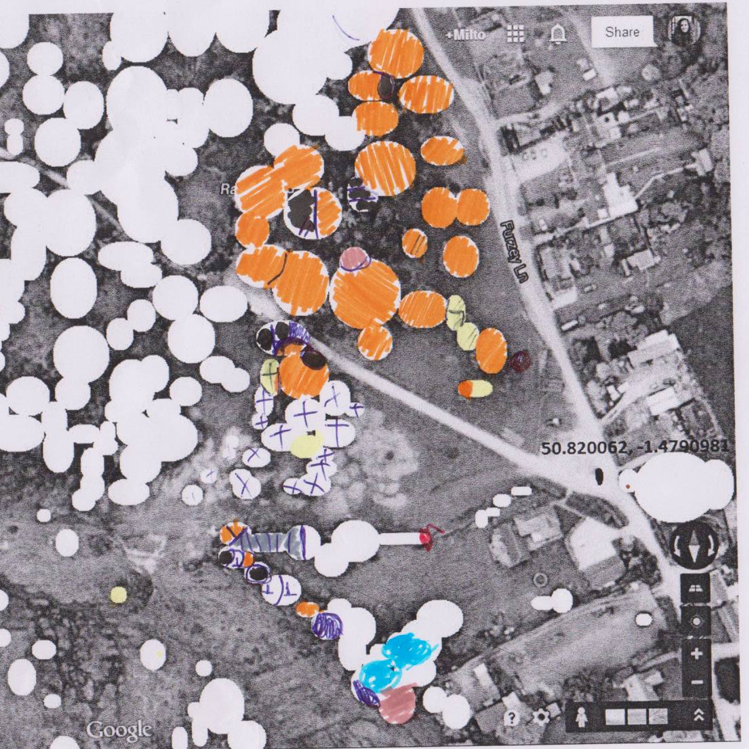
\includegraphics[width=.9\textwidth]{img/NewForest/Area2Fieldwork_Species}
	   		\caption{Tree species map, from field work}
	   		\label{fig:Area2Fieldwork_Species}
	   	\end{subfigure} \hfill
	   	\begin{subfigure}[t]{.5\textwidth}
	   		\centering
	   		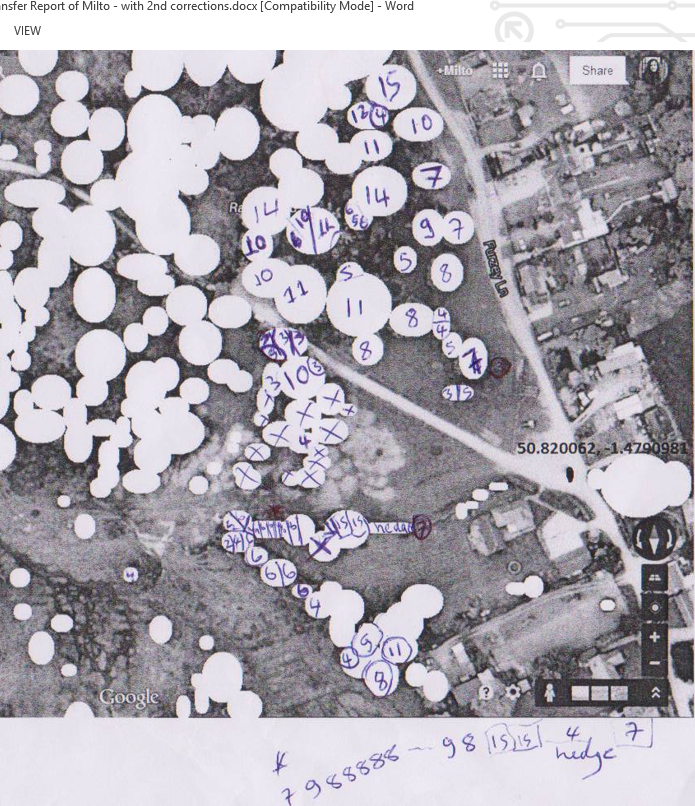
\includegraphics[width=.9\textwidth]{img/NewForest/Area2Fieldwork_Heights}
	   		\caption{Approximate heights of the trees, from field work} 
	   		\label{fig:Area2Fieldwork_Heights}
	   	\end{subfigure}
	   	\caption{The second area of interest and the related maps.} %\footnotemark[1].} 
	   	\label{fig:NF_Area2} 
	   \end{figure}
	   

   \newpage
\section{	Landscape types}
	During the forest assessment in New Forest, not only validation data were collected, but also useful information about classifying the data. The following images show examples of the five landscape types that were found in New Forest:
	
	1.	Heather fields:
    
      \begin{figure} [!h]
      	\centering
      	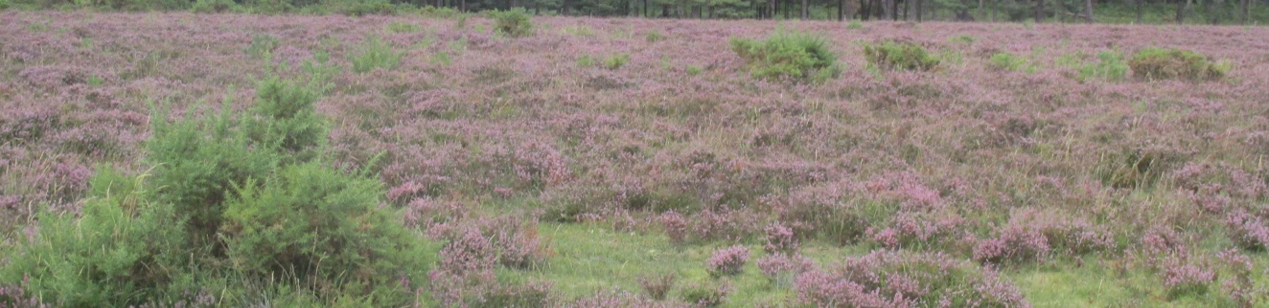
\includegraphics[width=\textwidth]{img/NewForest/LT_HeatherFields}
      	\caption{Trees that have been cut down}
      	\label{fig:LT_HeatherFields}
      \end{figure}

    
    2.	Grass with a few scattered trees:
          \begin{figure} [!h]
          	\centering
          	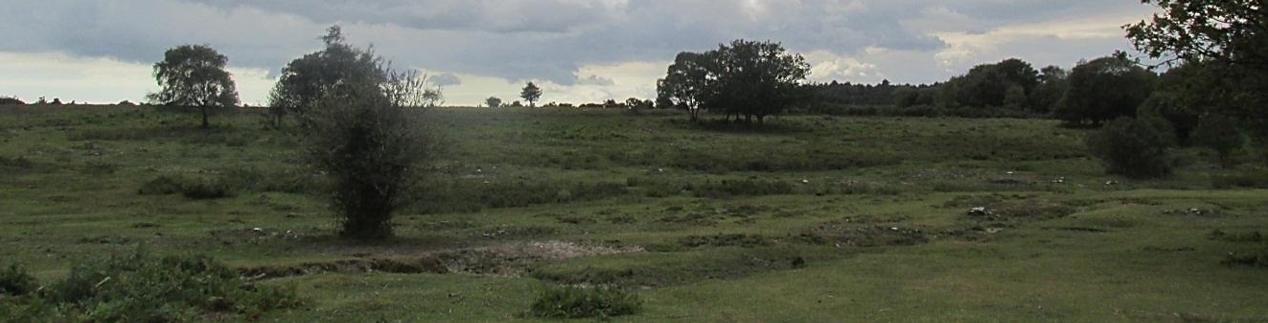
\includegraphics[width=\textwidth]{img/NewForest/LT_GrassWithFewTrees}
          	\caption{Grass with a few scattered trees}
          	\label{fig:LT_GrassWithFewTrees}
          \end{figure}

    3.	Dense Forest:
          \begin{figure} [!h]
          	\centering
          	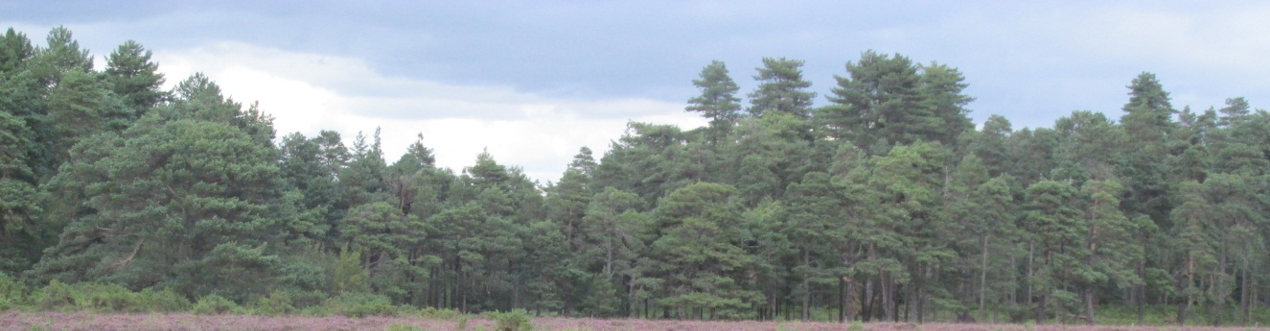
\includegraphics[width=\textwidth]{img/NewForest/LT_DenseForest}
          	\caption{Dense forest}
          	\label{fig:LT_DenseForest}
          \end{figure}
          
          \newpage
    
    4.	Bushes and Shrubs
          \begin{figure} [!h]
          	\centering
          	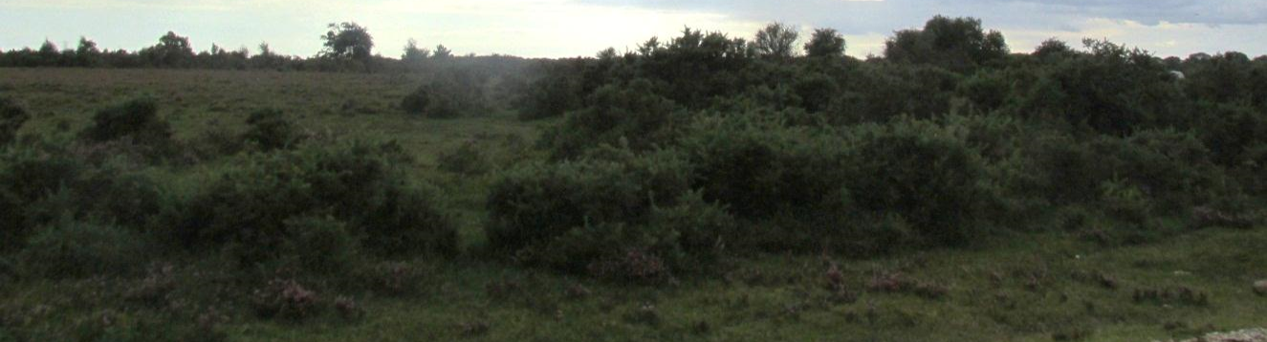
\includegraphics[width=\textwidth]{img/NewForest/LT_BushesAndShrubs}
          	\caption{Trees that have been cut down}
          	\label{fig:LT_BushesAndShrubs}
          \end{figure}

    
    5.	Lakes and rivers, which are more rarely found
          \begin{figure} [!h]
          	\centering
          	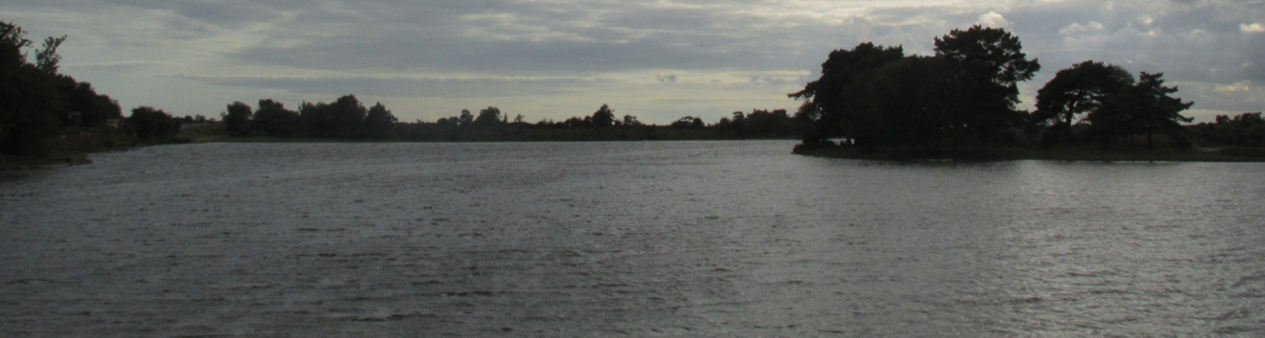
\includegraphics[width=\textwidth]{img/NewForest/LT_LakesAndRivers}
          	\caption{Lakes and rivers}
          	\label{fig:LT_LakesAndRivers}
          \end{figure}

    \par Please note that the landscape types could significantly differ according to the scanned area. For example, the landscape of New Forest is flat while the landscape of Eaves Wood (another scanned forest in UK) is hilly. The landscape type should be taken into consideration during classifications. 
    
    \subsection{Classification challenges}
    \par This case study brought further understanding of the challenges of creating validation data and writing a tree species classifier. These challenges are listed and explained below with some photos taken during field work:
    
    \par 1.	Field work and remotely sensed data collection should happen around the same time to avoid changes that happens over time. In the New Forest case, the airborne data were collected in 2010 and many changes occurred in the intervening time - in the most extreme cases, some trees had been cut down.
    
    \begin{figure} [!h]
    	\centering
    	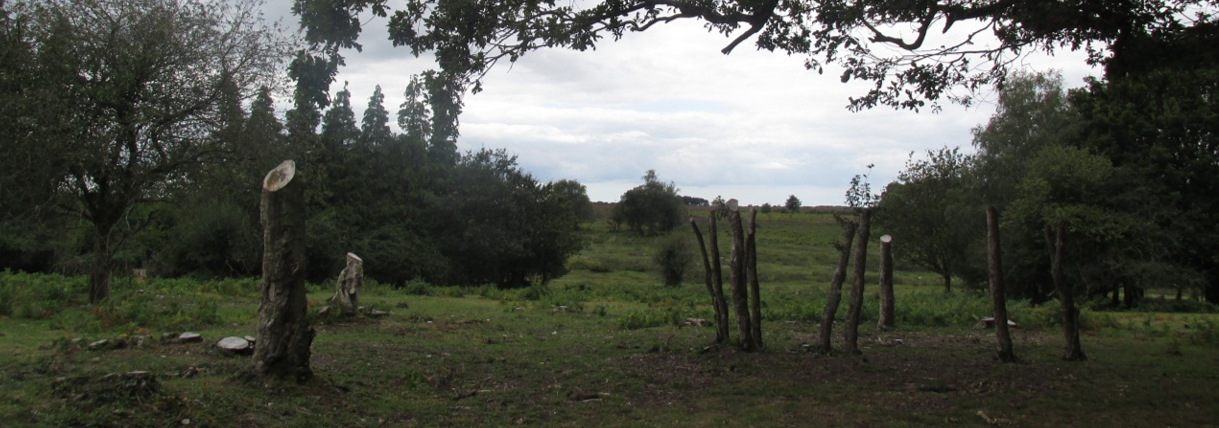
\includegraphics[width=\textwidth]{img/NewForest/CC_TreesCutDown}
    	\caption{Trees that have been cut down}
    	\label{fig:CC_TreesCutDown}
    \end{figure}

    \par 2. Machine learning becomes more time consuming as the number of classes increases. Regarding tree species classes, it is unrealistic to expect that all tree species will be identified.  This point is underlined by the fact that the list of tree species used in the tree assessment held by Sumnall \cite{Sumnall2013} didn’t include a number of trees (e.g. holly trees and crabapple) that were widespread in New Forest. 
    
    \par 3.	There is much more than just trees in the forest, including mobile animals, that may confuse a classification if LiDAR returns hit rocks, animals, vehicles or buildings instead of branches, leaves and trunks. {\color{blue} Any classification must account for inevitable errors due to background clutter that need to be invariant to. }
        \begin{figure} [!h]
        	\centering
        	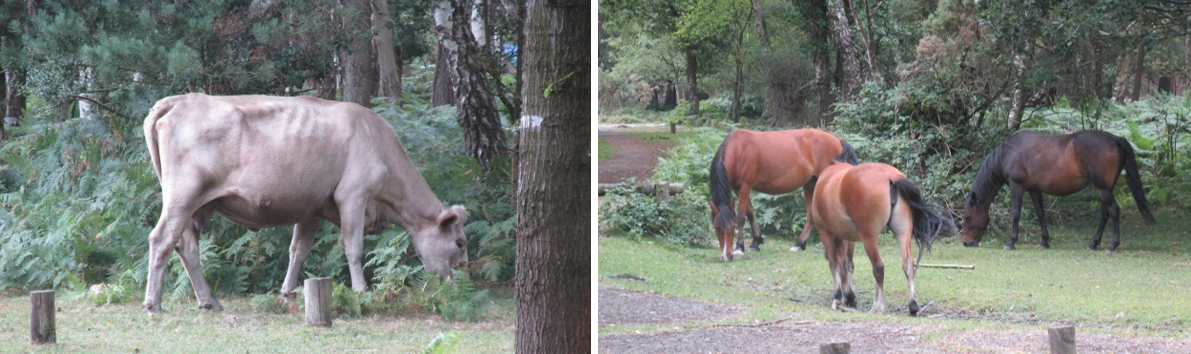
\includegraphics[width=\textwidth]{img/NewForest/CC_Animals}
        	\caption{Animals in New Forest}
        	\label{fig:CC_Animals}
        \end{figure}
    
    \par 4.	Large validation datasets from a single area will not be sufficient, because trees of the same species are usually gathered together. For instance, the first selected area has many pine trees while the second one has many oak trees. Therefore, it is important to have many field plots spread well within the area of interest.  
    
    \par 5.	Further, some trees are entwined together which makes it difficult to identify from the data whether they are one or two trees. Examples are shown in Figure \ref{fig:CC_MixedTrees}; in the left image, the trunks of the two trees are very close to each other and, in the right image, a crabapple and an oak tree have grown together. 
    
    \begin{figure} [!h]
    	\centering
    	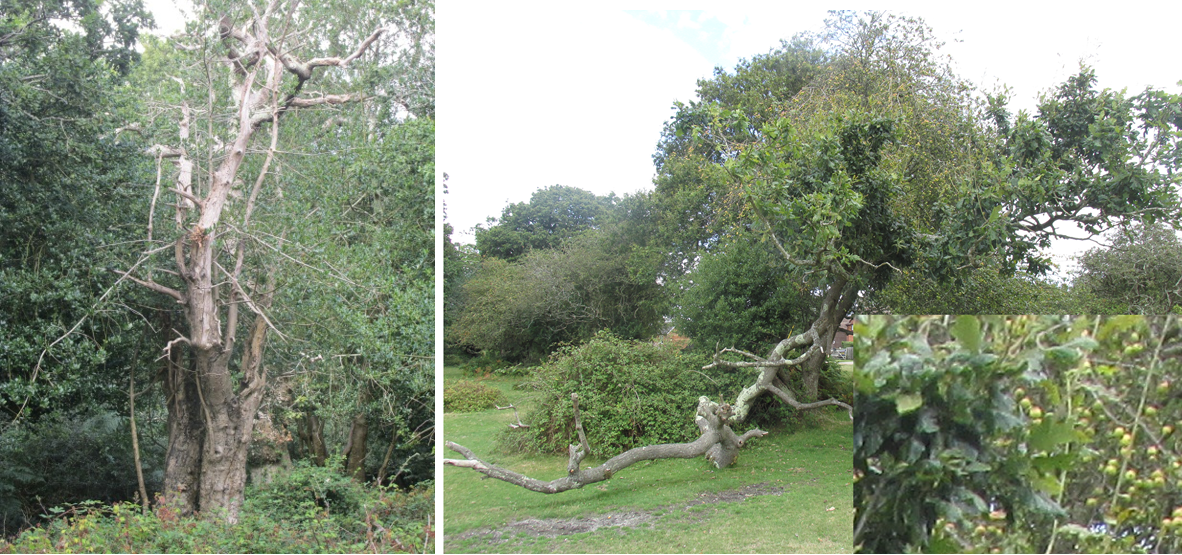
\includegraphics[width=\textwidth]{img/NewForest/CC_MixedTrees}
    	\caption{Trees, which are mixed together}
    	\label{fig:CC_MixedTrees}
    \end{figure}
    
    \section{Conclusions and Discussion }
    \par To sum up, the trip to the New Forest was essential for better understanding the challenges of remote monitoring of forests. During the visit, a small validation dataset was generated; the species and height of trees that are inside the two areas of interest were noted down. Field work is a time consuming task and weeks are required for generating a big enough validation dataset, but it is essential for understanding the object of interest (trees) in relation to the scanned data. Challenges identified were also explained and this increased knowledge about forests should lead to implementing a better classifier. 
    
\end{document}